\documentclass[12pt]{article}
\usepackage{uspstyle}
\usepackage{graphicx}

\begin{document}

\maketitle
\section*{Project}

% The content of your research proposal, including text, figures and images, 
% should not exceed 5 pages, typed, double-spaced (additional pages may be 
% included for your works-cited/references).

\section{Introduction}
% Provide a statement of the objective(s) and the anticipated significance of the 
% work to your field of study. What problems will be investigated? What hypothesis 
% will be tested? We suggest that the introduction begin with a brief description 
% of the project in general terms before the more technical aspects of the project 
% are discussed. 
%\todo{put some sort of high-level introduction here.}
%here is how you cite a figure (be sure to updated the ref here ... and the 
%label inside the figure

This project stems from the incredibly complicated biological system, metabolism. We were initially interested in verifying if the predicted rates of reactions are consistent with observation. However, through the lens of topological data analysis (TDA), we are optimistic we can not only accept or reject these current reaction rates for metabolism, but also more generally test physical models for self consistency and pinpoint which portion caused a failure. This is a huge step up from current methods for verifying models. As stated by K.P. Burnham and D.R. Anderson, ``Classical model testing is essentially limited to goodness-of-fit tests (which test only against an alternative hypothesis)" \cite{intro}. This is a considerable issue for multiple reasons. First, a system of this complexity is incredibly difficult to analyze in a standard fashion. Second, this method of model testing leaves out the possibility that most of the theory is correct. Under this regime, a system of fifty perfectly modeled reactions and one misrepresented one would result, provided it caused a significant margin of error, in a dismissal of the entire system. Obviously this is undesirable. This project in its finished state would allow us not only to methodically analyze any scale of complicated system, but also accept the fifty perfect reactions and further examine the remaining false one. The advantages of TDA are very clear - applying a testing framework that is far more versatile and informative is a huge advantage over the status quo.
%Figure~\ref{fig:TODO-name}

%TO cite something, use~\cite{fasy2014statistical}.

% \begin{figure}
%  \centering
%  \includegraphics[height=1.25in]{TODO:relative-path}
%  \caption{TODO.}\label{fig:TODO-name}
% \end{figure}

\section{Background}
% Provide a brief review of the work that has been done in the project 
% area together with complete references in appropriate professional style. This 
% section should also include any personal information about you that would 
% indicate to the reviewers your qualifications for successfully completing this 
% project, including a statement of how the project will contribute to your 
% academic and career goals.
%\todo{discuss related work, and why you are qualified to work on this.  Perhaps 
%make subsections.}
\subsection{Problem background}
Our approach utilizes the mathematical structure known as a sheaf. While they are traditionally very generally defined and used primarily in abstracting category and measure theory, we were inspired by the work of Michael Robinson and Brenda Praggastis to treat them as the ideal method for analyzing consistency in expansive sensor networks. Michael Robinson,  associate professor at American University, states ``Sheaf theory
provides a toolbox for constructing predictive models described by systems of
equations"\cite{mr}. This is precisely what metabolism is - a predictive model governed by a system of stoichiometric equations. Brenda Praggastis fleshes out this idea by explaining how to determine which portions of collected data is consistent with our predictions. Additionally, she mentions that given any system of equations, we can apply the same methodical sheaf structure to determine consistency \cite{pr}. This conclusion gives us the foundation to create an algorithm for solving this problem generally. Combining this baseline research, over the past summer we have been able to define a sheaf capable of determining consistency of measurable data (measurable quantities i.e., glucose), calculable data (aren't directly measured i.e., reaction rate), and are currently working on determining a metric to gauge which portion of our model is to blame for inconsistency. Additionally, we have obtained access to the "Pysheaf" code repository for sheaves, which will most likely
prove to be a very useful tool.

\subsection{Personal Value}
I am a Physics and Computer Science major who also enjoys math. Being involved in TDA at MSU during my undergraduate degree is extremely beneficial to me. I get the opportunity to learn an incredible amount of material, I get to work with fantastic and intelligent people, I get to enhance my public speaking and presentation skills, I learn techniques for high quality technical writing, and lastly, it prepares me for future vocation. All of these things will help secure a job and a position in graduate school, of which I am aspiring for both. 
\subsection{Qualifications}
I have been a part of the TDA group since early 2018. As such, I have built the foundations for doing research in the field, including participating in the spring semester of the course "Computational Topology," and participating in the group's summer reading session. However, my most convincing qualification is the fact that I have been working on this problem for the past summer and am starting already very familiar with the subject.


\section{Methods}
% Provide a detailed description of the research methods that you will 
% use in the project. This should include a justification for the specific 
% approach that you will use. For example, how do the methods answer the questions 
% that have been posed, test the hypothesis, or lead to the desired goal?
% Timeline: Provide dates for the initiation and completion of each phase of the 
% project. Attempt to lay out a reasonable schedule taking into consideration all 
% phases of the research and final deliverables.
\subsection{Methods}
In general, our method for creating this approach to model testing is summarized with TDA. More specifically, we plan to use a sheaf, which, as stated above, is particularly good at picking out locally consistent data. 
\begin{enumerate}
	\item Our first new goal is, given an inconsistent set of data, to determine which portion of our model is at fault. Using the tools laid out by linear algebra and sheaf theory, we hope to find a way to isolate the effects of each reaction. This would in turn allow us to easily pinpoint which reaction is at fault for causing an inconsistent measurement.
	
	\item  Our second goal includes writing code to solve this problem automatically. We have obtained the Pysheaf library, which has most of the tools we would want to use to model a sheaf in Python. 
	
	\item Future potential plans include determining acceptable error margins, confidence intervals on consistency, generalizing to nonlinear systems of equations, writing an algorithm to determine all of the above, and data simulation.
\end{enumerate}

\subsection{Example}
Below is an example of our sheaf applied to a very simple system of equations. With the sheaf framework, we can easily determine which portions of our model are consistent with observation (green), and which are not (red). Since we know our model is consistent for reactants A and C, we can assume our error is coming from some unaccounted for factor with B or an inaccurate reaction rate r1.  
\begin{figure}[h]
	\caption{\textit{Our sheaf applied to the reactions $A + B\rightarrow C$ at rate r1 and $C \rightarrow A$ at rate r2}}
	
	\centering
	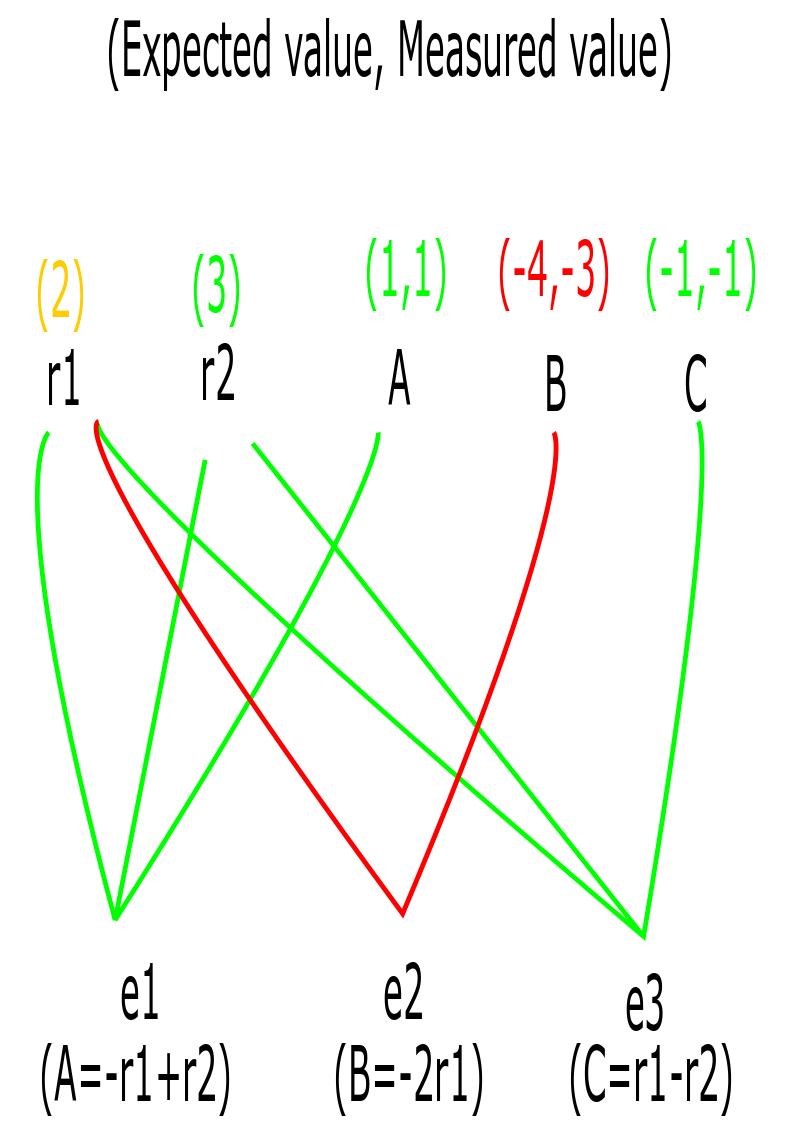
\includegraphics[width=0.5\textwidth, height=0.2\textheight]{USP2018f.PNG}
\end{figure}

\subsection{Timeline}
September: Work on goal one - determine which portion of our model is at fault.\\
October: Investigate acceptable error margins and confidence intervals. \\
November: Work on code and the writeup\\
December: Look into nonlinear systems and data simulation\\
January: Finish code and writeup\\
February: Prepare for Student Research Celebration in March
\section{Collaboration}
% Provide a description of the way you and 
% your faculty sponsor will collaborate on the project. The faculty sponsor should 
% play a significant role in responding to your ideas, providing advice for new 
% directions and resources, discussing the implications of the results, and 
% helping you prepare for your public presentation. Will there be regularly 
% scheduled meetings between you and your sponsor? Explain how the project relates 
% to the ongoing work of your sponsor, if this is the case.
In order to complete this project, I will be working very closely with my faculty advisor, Dr. Brittany Fasy. Additionally, I will be working with Anna Schenfisch, a graduate student in mathematics, and former MSU Post-Doctoral fellow Daniel Salinas. Our group will be meeting once a week on Tuesdays with exceptions of travel. 

%\todo{Does the following apply?  Report on Previous Research Experience (please 
%save and upload this as a 
%separate document): If you have done any previous research as an undergraduate 
%you must include a 1-2 page (double-spaced) summary of your research results or 
%creative products.Please note-if you have received funding from USP or INBRE 
%your proposal will not be considered unless you complete this section.}

% Please draft your proposal in a format that is appropriate for your academic 
% discipline (i.e. MLA, APA, etc.) - consult your mentor if you have questions 
% about what format is most appropriate to your field of study
%%%%%%%%%%%%%%%%%%%%%%%%%%%%%%%%%%%%%%%%%%%%
%% BIBLIOGRAPHY
 \newpage
 \bibliographystyle{acm}
 \begin{thebibliography}{widestlabel}
 \bibitem{pr}
Praggastis, Brenda. Maximal Sections of Sheaves of Data over an Abstract Simplicial Complex. ArXiv:1612.00397v1, 1 Dec. 2016.
\bibitem{mr}
Robinson, Michael. Sheaf and duality methods for analyzing
multi-model systems. arXiv:1604.04647v2 3 Nov. 2016.
\bibitem{intro}
Burnham K.P., Anderson D.R. (1992) Data-Based selection of an Appropriate Biological Model: The Key to Modern Data Analysis. In: McCullough D.R., Barrett R.H. (eds) Wildlife 2001: Populations. Springer, Dordrecht
 \end{thebibliography}


%%%%%%%%%%%%%%%%%%%%%%%%%%%%%%%%%%%%%%%%%%%%
% References Cited (include in an additional page within the project proposal): 
% Include a list of any literature that you have cited in the proposal. Nearly 
% all 
% good science and engineering proposals cite papers reporting related results, 
% describing the methods to be used or providing background information. Please 
% note-the review panel rarely recommends funding for proposals without adequate
% references.



\end{document}


